\section{Why NS3 was chosen and why it was dropped}

\section{Code Structure and Development Methodology}
	%Modular - each section should be self contained as far as possible
	%extensible - provide the minimum environment that can be extended into more useful programs
	%interconnecting - seems to conflict with modular, but is about creating common means of
	%				   communication between different parts of the program, e.g: broadcasting
	%				   works similarly to pushing new graphics to visualiser
	%Multi-threaded - Designed to emulate a physical deployment in that each section of the
	%				  simulator works independently of each other, best way to facilitate this was
	%				  use of multiple threads to simulate the components working simultaneously

	The simulator was created to be as modular as possible, each subsystem has very clearly defined
	links to the other parts of the simulator, for instance the methods of ``commMod" that interact
	with environment. Using this design allows for far easier modification and testing of each part
	of the system, as each part presents a ``contract" with the other pieces, so long as that ``contract"
	remains unchanged, the other parts of the system should be able to continue working identically
	to how they were before the changes. This also has benefits to possible optimisations of the system
	as any optimisations done, again, so long as they do not violate this ``contract" will be trivially
	intergratable.

	The simulator is extensible. This is actually the key to the way that the simulator works, the point
	of the simulator is that users will extend the provided classes to use the simulator, but this also
	allows users to extend the simulator in order to alter the way that the simulator works. As it is,
	the simulator is rather devoid of any non-essential features, but this is by design as the main problem
	with NS3, the simulator package that was going to be used for this project was feature bloat, causing
	the entire system to be unfocussed and thus more difficult to develop for than a more focussed system.

	Despite seemingly contradicting the first point of this section, the simulator is interconnecting,
	every system is related in some way to the others, Drone works very similarly to Base Station
	(which is to be expected, they both extend Messageable) the way that broadcasts work is very similar
	to the ability to push visualisation elements.

	Ultimately, the primary implementation decision was to use a lot of threads, this was to ensure that
	the system could emulate many independent machines at once, which is the primary purpose of the system.
	Unfortunately, this does lead to inefficiencies on machines with a lower number of available threads.

%Someone remind me to finish this -- Will
%Diagram of a simulation, with the environment, messageables, and commmods
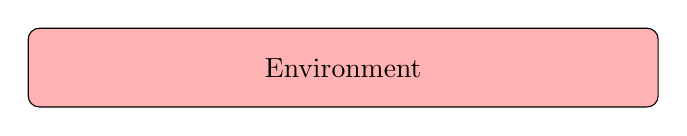
\begin{tikzpicture}
\filldraw[fill=red!30, draw=black, rounded corners] (0,0) rectangle (8,1);
\node at (4,0.5) {Environment};
\end{tikzpicture}

	\subsection{The Environment}
		The environment code is the central hub of the simulator, it handles all of the administration
		of the tasks being performed by the system. The environment contains all of the sample sensor
		data, and contains references to all of the messageable components of the simulation.

		The environment's thread is what can be seen as the ``main" thread of the system, this is the
		thread that handles the movement requirements of the drones as well as keeping track of the
		system's internal representation of time (which is independent of actual ``real-time" in that
		the internal time is a multiplier specified by the user of the total number of cycles that the
		environment thread has gone through).

		Another responsibility of the environment code is to handle the broadcasting of messages to
		the drones, this is achieved relatively inefficiently, using a simple collision detection
		method to check whether every known messageable is in range or not, this could be a target
		for optimisation for further development of the simulator, as will be outlined in the optimisation
		section below.

	\subsection{Communication Modules}
		Communications modules act as an intermediary between the messageables they are attached to and
		the environment in the simulator. In actual deployment, the communications modules can be seen as
		the lower-level network handling capabilities of the drone. The communications modules are implemented
		in such a way to reduce the workload of a developer creating messageable code, allowing for separation
		of labour into networking development and the actual programs to be executed on the messageables.

		Because of this, the communications modules primarily interface with the environment, passing messages
		to the attached messageable from the environment and messages from the messageable to the environment.

		In terms of actual functionality built in to the ``CommMod" class that represents the communications
		modules, it does little but pass messages and call the environment's ``broadcast" method. This is because
		the communications modules are not defined by the simulator but rather the user, allowing for custom
		communication protocols to be used.

		The only job of each communication module's thread is to run the supplied function until it terminates.

	\subsection{Messageables}
		``Messageable" is the superclass of all classes designed to be a destination for messages, in this case
		drones and base stations and all of their subclasses created by the user. The primary functions of the
		code in the ``Messageable" class is to contain the virtual methods to be overwritten by the user as
		well as some utility functions to facilitate communication between the running function of the messageable
		and its communication module.

		Each messageable's thread runs the user's overwritten function in the final subclass of the messageable.

		\subsubsection{Drone}
			Drone is a subclass of Messageable. The changes made to messageable with drone are simple, introducing
			new functions to facilitate the movement of the drone, as well as various utility functions to query the
			status of the drone, most of these functions are never called in the simulator itself, but rather are
			designed to be called by user defined subclasses of drone in the override of the ``run" function.

			Functions like ``move" do not actually cause the drone to move, but rather queue a movement for the drone
			that is then executed by the environment thread when the drone's ``upkeep" function is called.

		\subsubsection{Base Station}
			The ``Base Station" class is very simple as aside from a constructor change, it is just a type transformation
			over Messageable, this is mainly to simplify the experience for the end user as extending messageable to create
			a base station would be possible, but would have been confusing.

	\subsection{Visualisation}
		The visualisation system provided a large set of implementation issues. This is because of the multi-threaded nature
		of the simulator, different threads can push elements to be visualised at any point, these element pushes are mainly
		handled through several helper functions that each call an underlying element pushing function with preset arguments.
		This simplifies both the implementation and use of these functions. The issue with this method is that the element list
		can be polled to change at any time, even when the visualiser is in the middle of a drawing operation. Due to the way
		C++ iterators work, (and due to the fact that elements are removed when they have exceeded their ``lifespan") and the
		list of elements being removed from, this could cause iterators previously pointing to valid elements to become invalid.

		e.g: The element list consits of four elements, a base station, two drones and a broadcast. One of the drones is
		deactivated and thus removed from the element list, however the draw thread was drawing the broadcast at that exact
		moment. Because an element before the currently active element was deleted, the pointer to the active element becomes
		invalid. This means that the pointer can no longer produce a valid element, probably causing a segfault as unassigned
		memory is accessed.

		The solution to this problem was to lock both the ``step" function and the ``draw" function behind the same mutex lock.
		Effectively, this makes the two functions mutually exclusive, allowing only one of the two functions to be running at any
		given time. This causes any changes to the list of elements to be done only when there are not any active pointers to the
		list.

		The window management system used in visualisation was GLFW3, a platform independent system chosen due to its flexible
		nature and the fact that over systems like GLUT it can more easily handle multi-threaded applications.

\section{Potential Optimisations}
	This section will highlight several areas for optimisation, how they are inefficient and why they were written this way.
	The first and most obvious area for optimisation is in the environment code, in the way that broadcasting works. As the
	code is now, when a broadcast occurs, the entire list of messageables is tested, each one being checked whether it is
	within the range of the broadcast, if it is then the message is sent to that messageable. A potential optimisation 
	(especially for broadcast-heavy programs running on the simulator) would be to limit the messageables that receive the
	message to those in the general area of the broadcast perhaps through some kind of segmentation of the environment.

	Another area to be optimised could be the main threads calling of the upkeep functions on the drones, the way it works
	in the current implementation is that it calls upkeep one drone at a time. This works fine, but there are no dependencies
	between each drone's upkeep method, so parallelising this process could improve performance, though this would cause the 
	creation of even more threads (which this system already creates a lot of) so this optimisation could only be valid for
	systems that can afford to have a large number of threads running at once.

	These are the obvious systematic level optimisations that could be done, there are probably many more lower level
	optimisations as well as less obvious high level ones, also to be considered could be reducing the amount of threads
	that the system creates in order to improve performance on machines with less hardware threads (as switching the thread
	of execution can be expensive).

\section{Review Against Original Objectives}
	The only objective that pertains to this section is ``Implement a network simulator" which requires analysis as to whether
	the implemented system fulfills this objective. The objective requires a system that is capable of supporting the creation 
	of a network of drones which are capable of sending messages and reacting to messages they recieve. Due to the way that the
	system works, this requirement is fulfiled, arbirtary drone programs can be implemented on user defined Drone, CommMod and
	BaseStation subclasses.

	However, this objective also specifies ``Specifically tailored to our domain", this is where the analysis is required as
	the domain in which the project lies is flexible, in order to fulfil this objective the system would have to enable the
	creation of drone programs that can perform arbitrary tasks. The system fulfils this requrement too, the system was crafted
	specifically with this in mind, the simulator specified very little, causing no bottlenecks or restictions (with the exception
	of requiring exactly one base station).

\section{User Manual}
	In order to use the simulator, extend BaseStation once implementing the run and message\_callback methods and pass it to an
	instance of Environment created with the sample data for the simulation. From here, implement extensions to Drone and CommMod,
	one for each type of drone and communications module required, many projects will require only one of each of these, but it is
	possible that a project with multiple types of drones could be created. Instances of the created drones should be passed to
	the environment instance. In the run method for any Drone or BaseStation derived class, you may use the ``send\_message" method
	in order to send a message to the communications module for broadcasting, the ``wait\_for\_message" method in order to wait for
	the next incoming message (implementing the ``message\_callback" function allows for non-blocking communication) and use the
	``get\_time" and ``get\_position" methods to get the time and position respectively. Drone adds the functions ``move", ``turn",
	``getMaxSpeed", ``getSpeed", ``getAngle" and ``hasFinishedMoving" which return their respective values or do the obvious. The
	function ``sense" allows the drone to gather data of the supplied type.

	The ``CommMod" extensions allow the use of the ``broadcast" method as well as the ``pass\_message" method, with these sending
	messages into the environment and to the attached messageable respectively. The function of ``comm\_function" which should be
	extended by every extension of CommMod is the actual communication module code.

	The purpose of the simulator is the simulate the physical deployment of code on drones. The idea is that with a properly
	configured drone or base station, you can take the code in the simulator and run it on the actual drones and base stations
	with no work to port the code to the new machine.
